%===================================== CHAP 5 =================================

\chapter{Analysis}
\label{chap:analysis}
\todo[inline]{Make a table with baseline classification rate for logistic regression, put in our values. 1 Peer with no noise, 1 peer with noise, best case from other experiments that we want to highlight. This can lead to a discussion of why our results are not as good, where they show promise etc}
All prediction results given in this chapter are presented with mean and standard deviation values. These values are computed by evaluating each combination of parameters with 10-fold cross validation and taking the mean and standard deviation of accuracy across the 10 data folds.


\section{Baseline Classification results and comparisons}
\begin{table}[h]
	\begin{tabular}{ll}
		\begin{tabular}[c]{@{}l@{}}Error Rate/Spambase\end{tabular} &        \\
		Sharma\citep{sharma2013adaptive}                                    & 0.0103 \\
		Kumar\citep{kumar2012comparative}                                  & 0.1389 \\
		Our optimal result (Local model, no noise, 1 peer)                & 0.100  \\
		High privacy, few peers($\epsilon$=0.1, 10 peers)				  & 0.157  \\
		Aggregated model				                                  & 0.157  \\
		Ensemble model				                                      & 0.157  \\
		Less noise, more peers($\epsilon$=1.0, 100 peers)				  & xxx  \\
		Noisy result ($\epsilon$=0.1, 50 peers)                           & xxx  \\
		
		
	\end{tabular}
	\caption{Table with baseline results from the Adult Dataset}
	\label{tab:baseline_class_results_spambase}
\end{table}

\begin{table}[h]
\begin{tabular}{ll}
	\begin{tabular}[c]{@{}l@{}}Error Rate/Adult\end{tabular} &        \\
%	Krempl,Decision tree with bagging\citep{}                                    & 0.196 \\
	Logistic regression \citep{caruana2006empirical}   				  & 0.114 \\
	Pathak\citep{pathak2010diffprivhomo}                                & 0.24 \\	
	Our optimal result (Local model, e=1.0, 10 peer)                  & 0.157 \\
	High privacy, few peers($\epsilon$=0.1, 50 peers)				  & 0.163  \\
	Less noise, more peers($\epsilon$=1.0, 100 peers)				  & xxx  \\
	Noisy result ($\epsilon$=0.1, 50 peers)                           & xxx  \\
	Aggregated model														  & 0.185 \\
	Ensemble model													  &	0.165
	
	
\end{tabular}
\caption{Table with baseline results from the Adult Dataset}
\label{tab:baseline_class_results_adult}
\end{table}


These two tables form the baseline for the analysis of our classification framework. In Table \ref{tab:baseline_class_results_spambase} we have presented the results of two classifiers reported in the literature \cite{sharma2013adaptive,kumar2012comparative} for the Spambase dataset. These are both centralized approaches to logistic regression, where both had as a research goal of trying to find an ideal classifier for spam detection. In similar fashion, we provide two baseline classification results in Table \ref{tab:baseline_class_results_adult} for the Adult dataset. Here we chose to provide baselines for two approaches, where the first\cite{caruana2006empirical} is an optimal result using logistic regression in a centralized manner. The second entry is the result of the differentially private system of \cite{pathak2010diffprivhomo}, on which we've stated that we wish to improve in RQ3.




\todo[inline]{Expand upon our own baseline results, and compare them to the baselines found in literature}
\todo[inline]{Add a segway onto the next sections, so that we can discuss the importance of the different parameters in a natural way}

\section{Importance of epsilon}
As explained in section \ref{section:differential_privacy}, differential privacy works by disguising an individual's data in a dataset by adding noise to their records. The amount of noise added is determined by the privacy parameter  $\epsilon$, and grows exponentially the closer the parameter gets to zero. 

\begin{figure}[H]
	\centering
	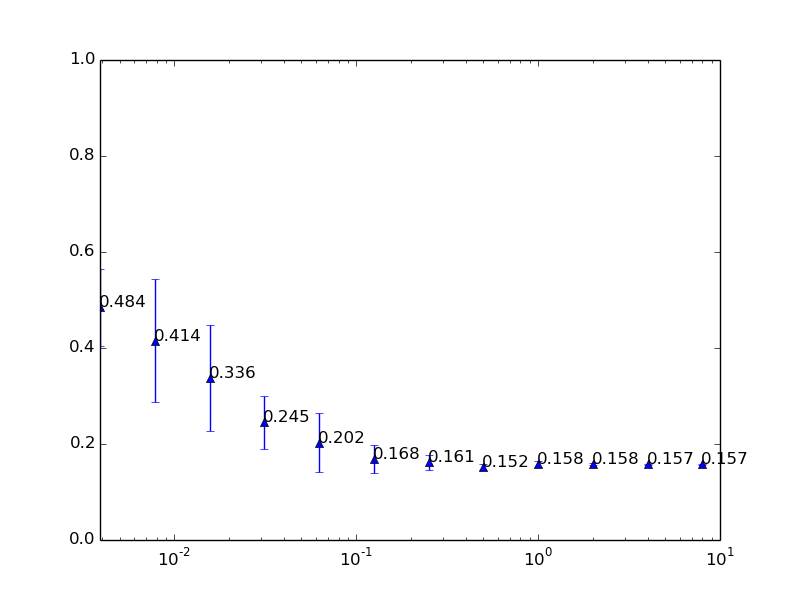
\includegraphics[width=\textwidth]{fig/spambase/eps2e-8-2e8,budg=eps,peers10,groups10,reg2e-2-data368-pubAll-spam-baseline-testset}
 	\caption{$\epsilon = [10^{-3}, 10^{3}], \lambda = 2^{-4}$, 50 peers, 1 aggregation}
 	\label{fig:epsilon_big_range}
\end{figure}
 
Figure \ref{fig:epsilon_big_range} shows the effect of the privacy parameter $\epsilon$ in our experiment. We wanted to test the effect of varying the $\epsilon$-value in the range from $2^{-10}$ to $2^9$, especially to find out how the classifier would perform when faced with data with high amount of noise added to it. The positive class rate in the UCI Spambase dataset is 0.4, so any error rate at this level is no better than a random classifier. The plot shows how sensitive output is to the values of $\epsilon$.

Figure \ref{fig:linear_epsilon_range} 

\section{The importance of data} \label{importance_of_data}
One of the more important findings for 
Data is important, the more data a peer have, the greater the chance is that it will make a decent local classifier. J

\begin{figure}[h!]
	\centering
	\begin{minipage}{.49\linewidth}
		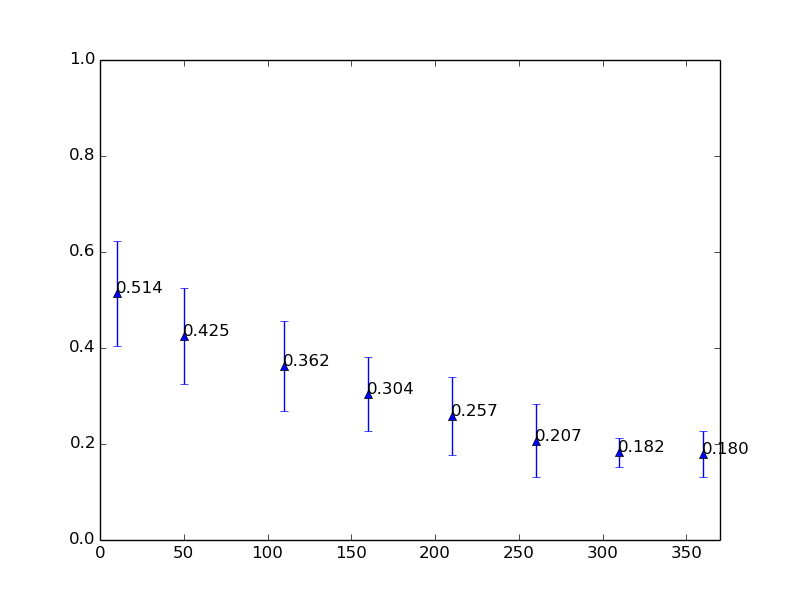
\includegraphics[width=\linewidth]{fig/spambase/eps0.1,budg=eps,peers10,groups10,reg2e-2-pubAll-spam-baseline-data10-360-testset-withoutlocalmodel}
		\captionof{figure}{$\epsilon = 0.1, \lambda = 2^{-2}$, 10 peers, 1 aggregations. Aggregated model only.}
		\label{fig:data_limit_test_withoutlocalmodel}
	\end{minipage}
	\hspace{.001\linewidth}
	\begin{minipage}{.49\linewidth}
		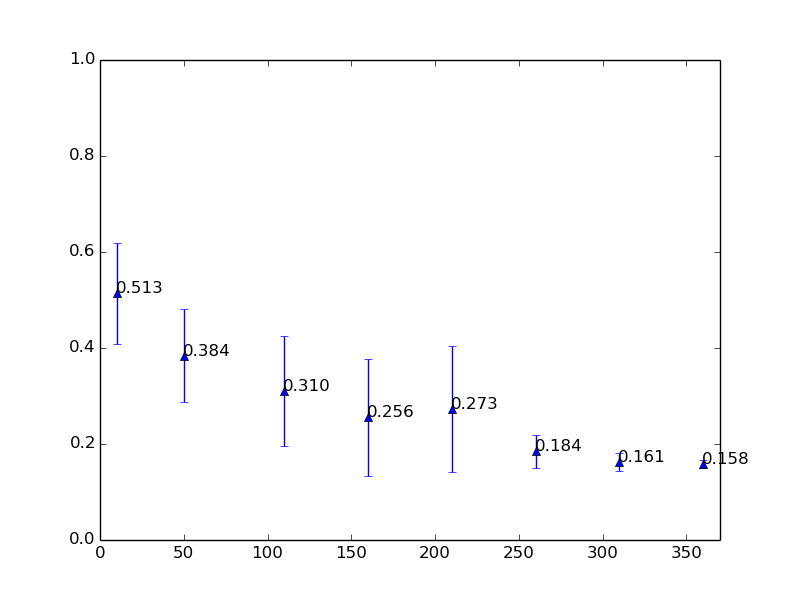
\includegraphics[width=\linewidth]{fig/spambase/eps0.1,budg=eps,peers10,groups10,reg2e-2-pubAll-spam-baseline-data10-360-testset-withlocalmodel}
		\captionof{figure}{$\epsilon = 0.1, \lambda = 2^{-2}$, 10 peers, 1 aggregation. Aggregated and local model.}
		\label{fig:data_limit_test_withlocalmodel}
	\end{minipage}
	\begin{minipage}{.49\linewidth}
		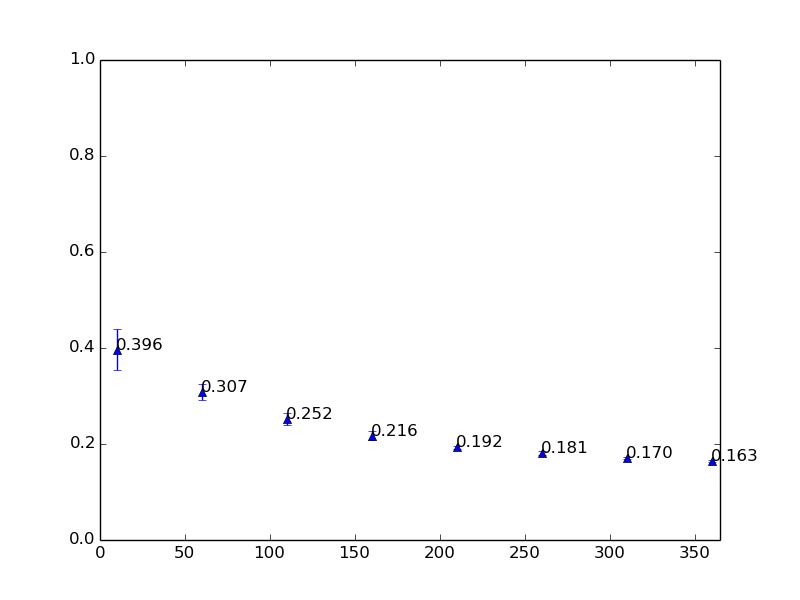
\includegraphics[width=\linewidth]{fig/spambase/eps0.1,budg=eps,peers10,groups10,reg2e-2-pubAll-spam-baseline-data10-360-testset-localmodelonly}
		\captionof{figure}{$\lambda = 2^{-2}$, 10 peers, local model only.}
		\label{fig:data_limit_test_localmodelonly}
	\end{minipage}
\end{figure}

\todo[inline]{Compare the figures about data limits, ie datalimittestwithoutlocalmodel and such. Clearly, with local model is better than without, but it is not clear whether local only or aggregated+local is better.}

Figure \ref{fig:data_limit_test} indicate how the classification performance improves as the amount of data records available to each peer grows. When each peer only have a small amount of data to create their local classifier, the classifier tends to have display terrible performance. As peers gain more data, both the performance and the variance of the classifier improves.     

The reason for this improvement is two-fold. 1: A bigger sample size for the logistic regression model generally leads to better performance \cite{peduzzi1996simulation}. 2: The sensitivity of logistic regression (see equation \ref{eq:logres_sensitivity}) is bounded by the size of the training set. What this means is that the more data a peer have available, the less amount of noise is needed to obfuscate their logistic model. 

The observation we've made is therefore thoroughly grounded in theory, and is important to highlight when discussing our main research question. Until a certain amount of data has been gathered, a system based on our distributed architecture will display very poor performance. What is interesting however, is that the amount of data needed seems to be a relatively low number. In the paper written by \cite{pathak2010diffprivhomo}, they report that each party was given at least 3256 data records. In our experiments we found that a much smaller amount of data could still be used and create decent classifiers. We believe this is due to our choice of propagating every model out, so that each peer can create an ensemble of classifiers. \todo[inline]{Fix this last sentence. It is not that good}

\section{Importance of regularization}

\begin{figure}[h!]
	\centering
	\begin{minipage}{.49\linewidth}
		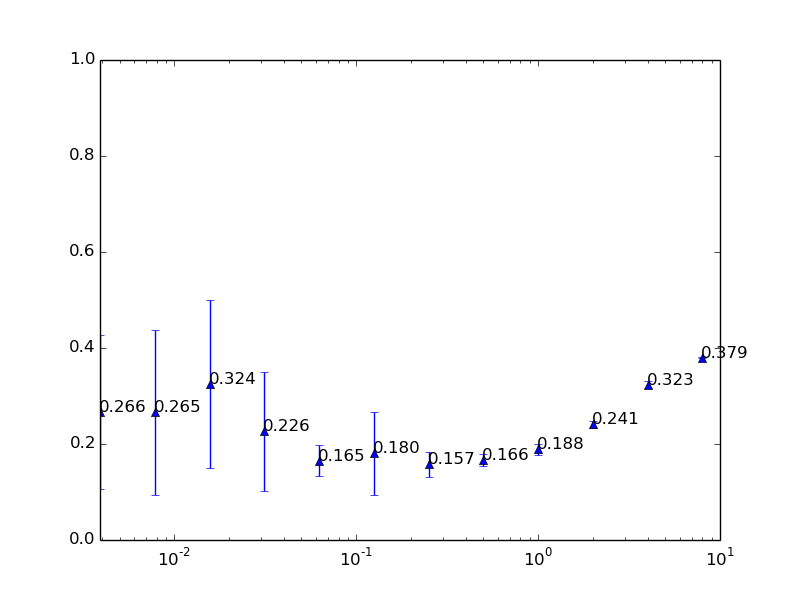
\includegraphics[width=\linewidth]{fig/spambase/eps0.1,budg=eps,peers10,groups10,reg2e-8-2e3-data368-pubAll-spam-baseline-testset}
		\captionof{figure}{$\epsilon = 0.1, \lambda = [2^{-8}, 2^{3}]$, 10 peers, 1 aggregation}
		\label{fig:regularization_normalepsilon}
	\end{minipage}
	\hspace{.001\linewidth}
	\begin{minipage}{.49\linewidth}
		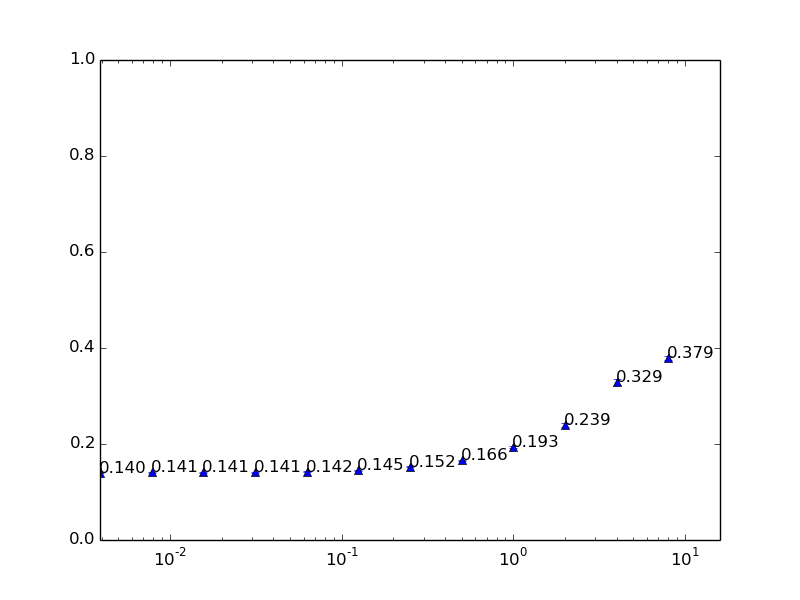
\includegraphics[width=\linewidth]{fig/spambase/eps2e10,budg=eps,peers10,groups10,reg2e-8-2e3-data368-pubAll-spam-baseline-testset}
		\captionof{figure}{$\epsilon = 2^{10}, \lambda = [2^{-8}, 2^{3}]$, 10 peers, 1 aggregation}
		\label{fig:regularization_extremelyhighepsilon}
	\end{minipage}
\end{figure}

Figure \ref{fig:regularization_extremelyhighepsilon} shows the normal effect regularization has on accuracy for the spambase data set, by setting $\epsilon$ so high that noise is essentially nonexistent. As the regularization parameter $\lambda$ grows large, the model becomes less able to fit the training data, eventually resulting in models predicting only the negative class, which constitutes 60\% of the data set. This happen because the high regularization forces the parameter vector to the zero vector, resulting in uniform class probability for all samples. 

On this particular dataset it appears that a logistic regression model is not at risk of overfitting, since the cross validated error does not increase when the level of regularization is very low. Ignoring the effects of privacy mechanisms, this would mean that selecting some regularization parameter in the range $[10^{-5},10^{-2}]$ could be acceptable. Choosing a level at the high end of this range could be a good idea, to reduce the risk of overfitting

Figure \ref{fig:regularization_normalepsilon} shows mean accuracy over a range of $\lambda$ similar to Figure \ref{fig:regularization_extremelyhighepsilon}, where $\epsilon$ is set to a level where the noise variance still has an effect on prediction accuracy, as seen in figure \ref{fig:epsilon_big_range}.

When noise with significant variance is added to the model creation process, tuning $\lambda$ will adjust noise variance as well. Equation \ref{eq:aggregated_logistic_sensitivity} states that the noise variance is inversely proportional to $\lambda$. The choice of regularization then must balance the model flexibility at lower levels of $\lambda$ with the decreased noise at higher levels of lambda.

\todo[inline]{Talk about how it is interesting that regularization now must respect something other than just model performance, and offer some guidelines on how regularization should be considered, especially in a setting like ours, with many independent parties}

\subsection{Analysis of Propagation and group size}

\todo{Add some subsection that talks about the effect on standard deviation among peers, and give the numbers from table used in our presentation.}

As mentioned in Section \ref{sec:PropagationPubModel}, we hypothesized that we could improve the overall classification accuracy of our system by publishing the aggregated models generated in phase 2.\unsure{Rewrite this if we don't use phases} In this section we present the effects of publishing method. Figure \ref{fig:RegRangeTestPubParty} shows the case where each group of peers only share the perturbed, aggregate model among themselves, while Figure \ref{fig:RegRangeTestPubAll} shows the results the model is sent to all existing peers. 

The most obvious effect of globally publishing models is that the standard deviation is much lower than the group publishing case. This is not surprising.

\begin{figure}[H]
	\centering
	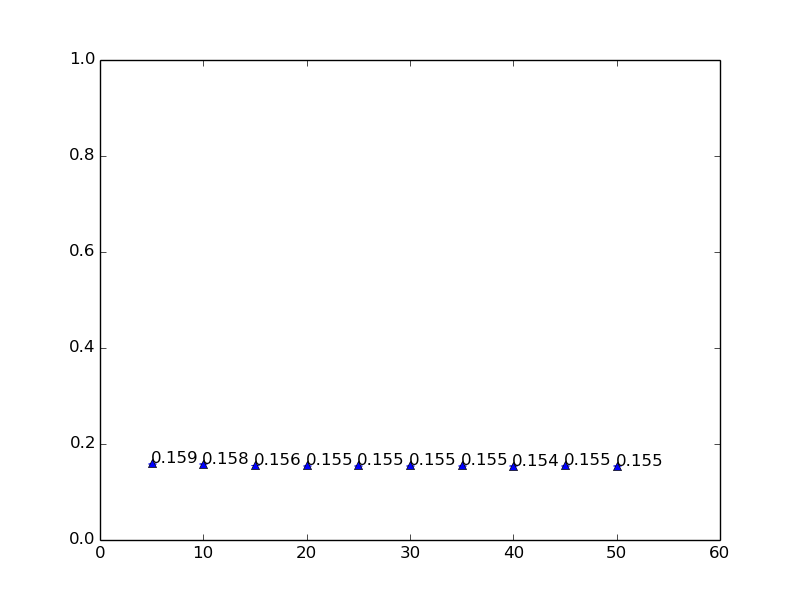
\includegraphics[width=\textwidth]{fig/adult/eps1.0,budg=eps,peers5-55,groups5,reg2e2-data500-pubAll-adult-groupbypeerverification-3-testsetmean}
	\caption{Effect of peer numbers. Group size: 50. Publishing: All. Data: 500}
	\label{fig:peer_range_constant_group}
\end{figure}

Figure \ref{fig:peer_range_constant_group} shows what happens when the aggregation group size stays fixed, but different numbers of peers are available. A higher number of peers mean that more models. In this experiment the aggregation group size was five, which means that just one aggregated model was produced at the low end of the range, while 10 models were produced at the high end. If there is any utility of aggregating models, it is not visible in the mean error rate for the Adult data set with this amount of records. We suspected that an effect would be stronger when the peers have less data, since aggregation should allow the peers to benefit from each other data. We tested with different amounts of available data as low as 75 instances per peer, but we made the same observations in these. The charts showing other levels of data availability are included in the Appendix.  \todo[inline]{Add figures to appendix that show our other tests}.

On the flip side, there doesn't appear to be any negative effects of predicting with an ensemble of aggregated models. \todo{Talk more about this}

One possible explanation for the small changes in error rate might be the uniform. This is discussed further in Section \ref{sec:Future Work} on Future Work.  

The truth is probably somewhere in the middle - we can't expect to easily publish models globally in all settings. Additionally, there might be situations were global publishing could be detrimental to real world performance - for instance, if there are strong geographical, temporal or demographic trends, it might be better to limit the amount of model sharing to suitable subsets.

\todo[]{Replace this figure with table showing std numbers and performance for a particular regularization isntead.}
\begin{figure}[h!]
	\centering
	\begin{minipage}{.49\linewidth}
		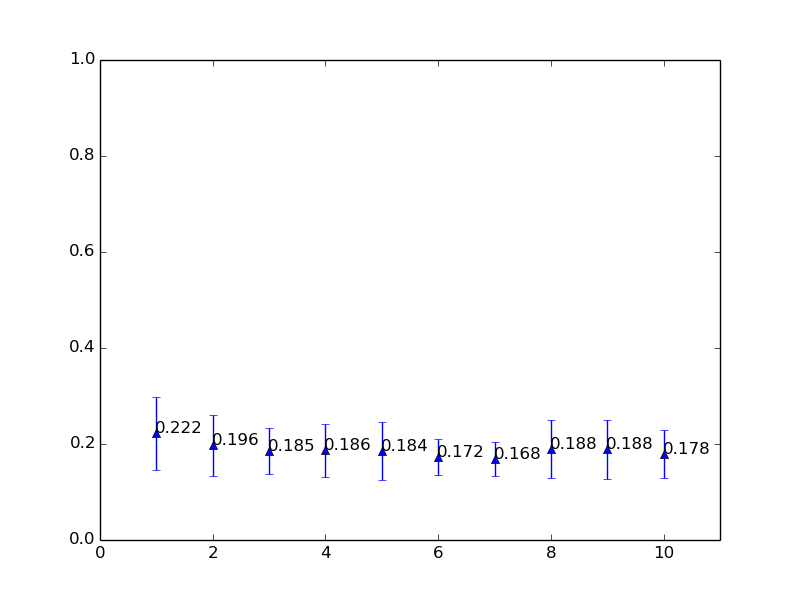
\includegraphics[width=\linewidth]{fig/PartyAllComparisonSpam-eps1.0,budg=eps,peers30,groups1-10,reg2e-2-pubParty-newAggregationStyleTEST.png}
		\captionof{figure}{$\epsilon = 1.0, \lambda = [2^{-5}, 2^{4}]$ 50 peers, 25 aggregations, publish to participants}
		\label{fig:RegRangeTestPubParty}
	\end{minipage}
	\hspace{.001\linewidth}
	\begin{minipage}{.49\linewidth}
		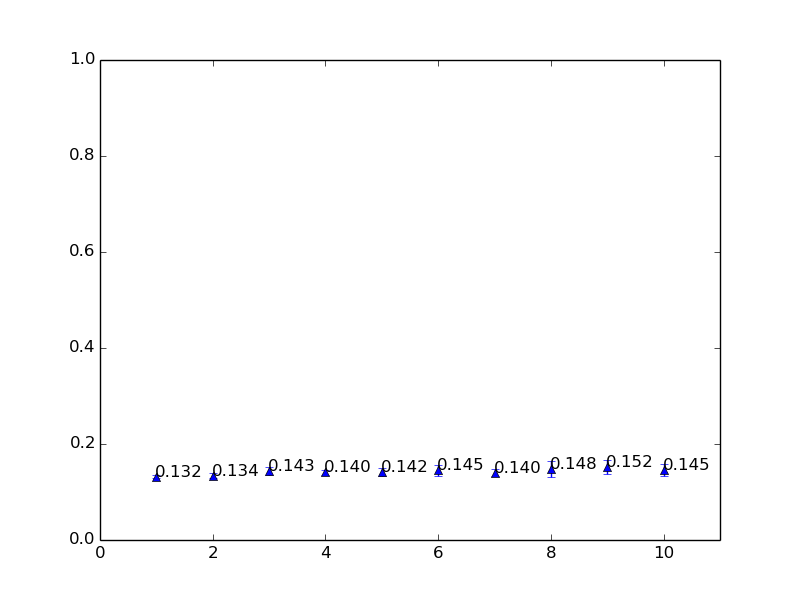
\includegraphics[width=\linewidth]{fig/PartyAllComparisonSpam-eps1.0,budg=eps,peers30,groups1-10,reg2e-2-pubAll-newAggregationStyleTEST.png}
		\captionof{figure}{$\epsilon = 1.0, \lambda = [2^{-5}, 2^{4}]$ 50 peers, 25 aggregations, publish to all}
		\label{fig:RegRangeTestPubAll}
	\end{minipage}
\end{figure}


As the previous experiment indicates that publishing newly made models to as many peers as possible is better \todo{Add a reflection talking about why this makes sense.}, we performed an additional experiment to determine whether it in such a scenario would be better to perform many aggregations with fewer models included in each aggregate or performing few aggregations including many models. This was achieved by testing performance with a range of values. In the experiment, each peer can only participate in a single aggregation before reaching the limit set by the privacy guarantee. For example, given a set of 50 peers, a aggregation size of 25 can only publish two aggregated models.
 
\begin{figure}[h!]
	\centering
	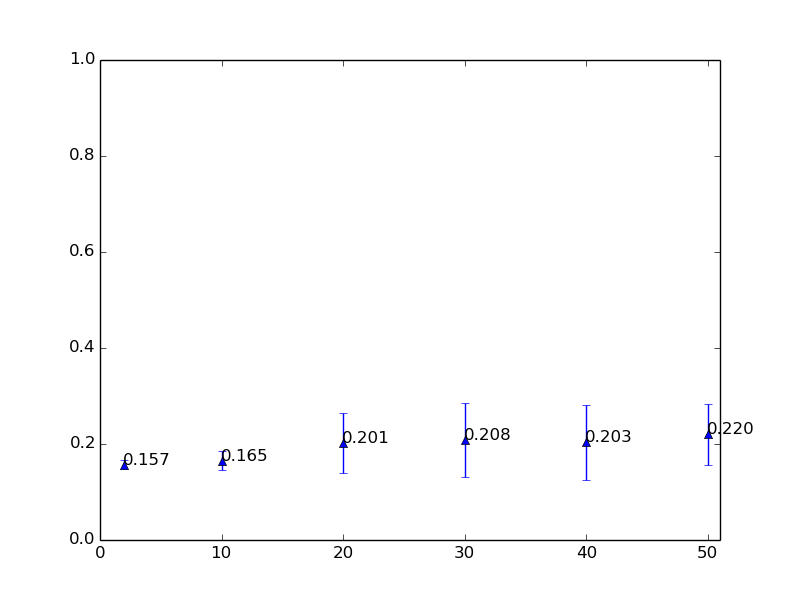
\includegraphics[width=\textwidth]{fig/GroupSizeEffectSpam-eps1.0,budg=eps,peers50,groups2-50,reg2e0-pubAll-LRbyCV-retuning}
	\caption{Spambase. $\epsilon = 1.0, \lambda = [1.0]$, 50 peers, aggregation sizes in range [2, 50], 66 samples per peer}
	\label{fig:groupsize_is_better}
\end{figure}

The results of this experiment is seen in Figure \ref{fig:groupsize_is_better}. It is clear that a smaller group size and consequently more aggregated models published resulted in a strong reduction in accuracy variance. While the variance is too high at larger group sizes to know much about the actual mean value after only 10 repetitions of the experiment, it is unlikely that it is smaller than the mean accuracy observed when the group size is one. 

A possible explanation of this result is that the effects of \unsure{bagging?} boosting counters the loss in accuracy that results from the addition of noise. Since models will have noise added to them before being published, expending all data to produce a single model might yield a worse classifier than partitioning data, adding noise to each separate, weaker model and combining them in an ensemble. On the other hand, this effect could be caused by some leakage of privacy which becomes visible over repeated applications of the aggregation mechanism. \todo{Figure out if there is some way we could test or prove that this is not the case.} 

The interesting observation that can be made from this is that the best situation is when there is no aggregation. A group size of one results in only a single model being contributed, and is equivalent to each peer publishing its local model with noise. One possible reason for this could be that there simply is no value in averaging models in the way done in our experiments and by Pathak et al.\cite{pathak2010diffprivhomo}. Neither our experiment or the experiment by Pathak et al. help distinguish between these two possibilities. The experiment by Pathak et al. only demonstrate that their method for creating aggregated models has comparable performance to adding noise to a centrally computed model. Additionally, this is only demonstrated with large data sets. In their experiment, the minimum data set size for any participant is 3256. With data sets this large, it is possible they would have gotten similar results by testing a model produced by a single participant, without performing additional aggregation. However, no experiment evaluating this possibility remains. Their theoretical conclusions stand, but experimentally validating the value of aggregation is necessary.

Thus the key question is whether or not aggregation is worth the complexity of a homomorphic encryption protocol. If similar performance can be achieved solely by ensemble classifiers of differentially private models published by each peer, one could skip the complexity and risk of relying on a cryptographic protocol to maintain privacy.

Another possible explanation for this observation is that aggregation might be useful, but not when the peers all have samples of data from the exact same distribution. This is the case with the Spambase data set used in the experiment in Figure \ref{fig:groupsize_is_better}.

One way to answer question would be by finding a data set which has subsets that are produced by distinct distributions, and partitioning data by source distribution. Due to time constraints we did not have time to locate and prepare data sets that fit this requirement. \todo{See if we have time to do this. We REALLY sho1uld, otherwise it will very possibly give a lower grade.}

\begin{figure}[h!]
	\centering
	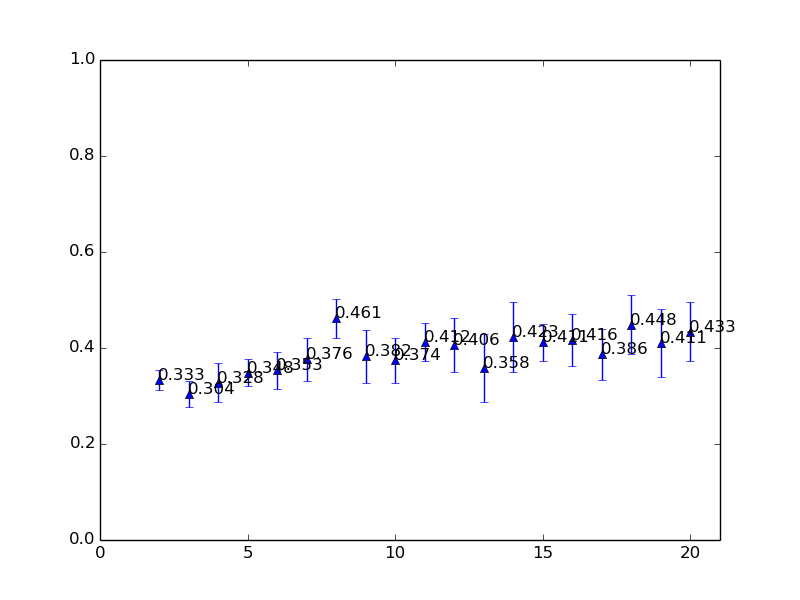
\includegraphics[width=\textwidth]{fig/spambase/ShowingPotentialUsefulnessOfLargerGroups-eps1.0,budg=eps,peers50,groups2-20,reg2e-2-dataMax20-pubAll-LRbyCV-retuning}
	\caption{Spambase. $\epsilon = 1.0, \lambda = [1.0]$, 50 peers, aggregation sizes in range [2, 50], 20 samples per peer}
	\label{fig:groupsize_limiteddata}
\end{figure}


An alternative avenue for validating the value of doing aggregation could be to reduce the amount of data given to each peer. If just one peer has data sufficient to train a good classifier, it is sufficient. For that reason it makes sense to stage a situation were it is highly unlikely that even a single peer gets a lucky subset of data. Figure \ref{fig:groupsize_limiteddata} demonstrates such a case. Again, there is not clear indication that averaging multiple models is better than simply publishing them individually and using them in ensemble classifiers.

\todo[inline]{redo this experiment above with regularization=0, as indicated by the previous figures shown}

%\subsection{Issues with cold start}
%
%Section \ref{sec:} important motivation for this project was the idea that application users should be able to retain ownership of their own data, and only share it to a degree that they choose.
%
%
%\todo[inline]{Explain what cold start issues is. Discuss how this is very prominent in our sitaution, and the different ways we can deal with the cold start, and pros and cons of those approaches. Essentially, we have already experimented with a kind of cold start situation when we try to performance numbers for peer\_count 1 to 50}
%








\cleardoublepage